% !TeX spellcheck = pl_PL
% Options for packages loaded elsewhere
\PassOptionsToPackage{unicode}{hyperref}
\PassOptionsToPackage{hyphens}{url}
%
\documentclass[a4paper,11pt]{article}
\usepackage{times,fullpage,polski}
\usepackage{amssymb,amsmath}

 \usepackage[T1]{fontenc}
\usepackage[utf8]{inputenc}
\usepackage{textcomp} % provide euro and other symbols


%\usepackage{ifxetex,ifluatex}
%\ifnum 0\ifxetex 1\fi\ifluatex 1\fi=0 % if pdftex
%  \usepackage[T1]{fontenc}
%  \usepackage[utf8]{inputenc}
%  \usepackage{textcomp} % provide euro and other symbols
%\else % if luatex or xetex
%  \usepackage{unicode-math}
%  \defaultfontfeatures{Scale=MatchLowercase}
%  \defaultfontfeatures[\rmfamily]{Ligatures=TeX,Scale=1}
%\fi
%% Use upquote if available, for straight quotes in verbatim environments
%\IfFileExists{upquote.sty}{\usepackage{upquote}}{}
%\IfFileExists{microtype.sty}{% use microtype if available
%  \usepackage[]{microtype}
%  \UseMicrotypeSet[protrusion]{basicmath} % disable protrusion for tt fonts
%}{}
%\makeatletter
%\@ifundefined{KOMAClassName}{% if non-KOMA class
%  \IfFileExists{parskip.sty}{%
%    \usepackage{parskip}
%  }{% else
%    \setlength{\parindent}{0pt}
%    \setlength{\parskip}{6pt plus 2pt minus 1pt}}
%}{% if KOMA class
%  \KOMAoptions{parskip=half}}
%\makeatother
%\usepackage{xcolor}
%\IfFileExists{xurl.sty}{\usepackage{xurl}}{} % add URL line breaks if available
\IfFileExists{bookmark.sty}{\usepackage{bookmark}}{\usepackage{hyperref}}
\hypersetup{
  hidelinks}
\urlstyle{same} % disable monospaced font for URLs
\usepackage{graphicx}
%\makeatletter
%\def\maxwidth{\ifdim\Gin@nat@width>\linewidth\linewidth\else\Gin@nat@width\fi}
%\def\maxheight{\ifdim\Gin@nat@height>\textheight\textheight\else\Gin@nat@height\fi}
%\makeatother
%% Scale images if necessary, so that they will not overflow the page
%% margins by default, and it is still possible to overwrite the defaults
%% using explicit options in \includegraphics[width, height, ...]{}
%\setkeys{Gin}{width=\maxwidth,height=\maxheight,keepaspectratio}
%% Set default figure placement to htbp
%\makeatletter
%\def\fps@figure{htbp}
%\makeatother
%\setlength{\emergencystretch}{3em} % prevent overfull lines
%\providecommand{\tightlist}{%
%  \setlength{\itemsep}{0pt}\setlength{\parskip}{0pt}}
%\setcounter{secnumdepth}{-\maxdimen} % remove section numbering


\newcommand{\ang}[1]{(ang. \emph{#1})}


\begin{document}


\title{Kwantowe obliczenia wariacyjne\\ {\normalsize Zastosowania}}

\author{Jarosław Miszczak}
\date{21/12/2022}

\maketitle

\begin{abstract}
Raport przedstawia wybrane zastosowania wariacyjnych algorytmów kwantowych. 
\end{abstract}


%-------------------------------------------------------------------------------
\hypertarget{wprowadzenie}{%
\section{Wprowadzenie}\label{wprowadzenie}}
%-------------------------------------------------------------------------------


\newpage 

%-------------------------------------------------------------------------------
\hypertarget{zastosowania}{%
	\section{Zastosowania}\label{zastosowania}}
%-------------------------------------------------------------------------------


\begin{figure}[ht!]
	\centering
	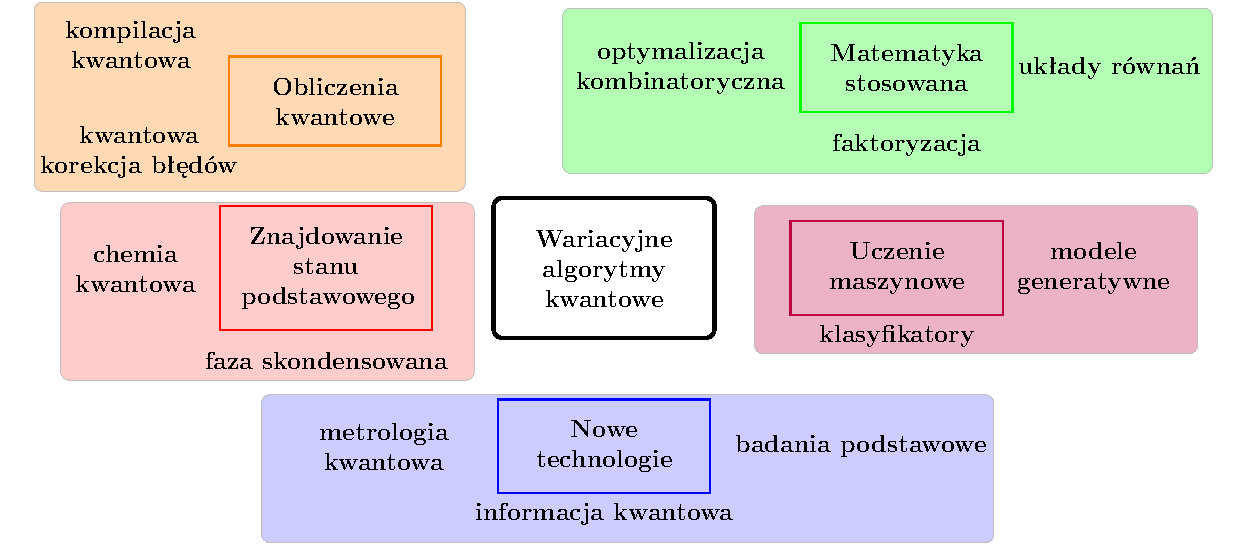
\includegraphics[width=\textwidth]{vqa-applications-pl}
	\caption{Potencjalne dziedziny w których zastosowanie wariacyjnych algorytmów kwantowych może prowadzić do uzyskania przewagi kwantowej.}
\end{figure}

%-------------------------------------------------------------------------------
\hypertarget{matematyczne}{%
	\subsection{Problemy obliczeniowe}\label{matematyczne}}
%-------------------------------------------------------------------------------

%-------------------------------------------------------------------------------
\hypertarget{sec1}{%
	\section{sec1}\label{sec1}}
%-------------------------------------------------------------------------------




\paragraph{}
\paragraph{}
\paragraph{}
\paragraph{}





%-------------------------------------------------------------------------------
\subsection{}
%-------------------------------------------------------------------------------


%-------------------------------------------------------------------------------
\subsection{}
%-------------------------------------------------------------------------------

%-------------------------------------------------------------------------------
\subsection{}
%-------------------------------------------------------------------------------




\newpage 

\hypertarget{literatura}{%
\section*{Literatura}\label{literatura}}

\begin{enumerate}
\def\labelenumi{\arabic{enumi}.}
%\tightlist

\subsection*{Rozwiązywanie układów równań}

\item Huang, H.Y., Bharti, K. and Rebentrost, P., 2021. Near-term quantum algorithms for linear systems of equations with regression loss functions. New Journal of Physics, 23(11), p.113021. \url{https://doi.org/10.1088/1367-2630/ac325f}


\item Bravo-Prieto, C., LaRose, R., Cerezo, M., Subasi, Y., Cincio, L. and Coles, P.J., 2019. Variational quantum linear solver. LA-UR-19-29101, arXiv:1909.05820. \url{https://doi.org/10.48550/arXiv.1909.05820}

\item Pellow-Jarman, A., Sinayskiy, I., Pillay, A. et al. A comparison of various classical optimizers for a variational quantum linear solver. Quantum Inf Process 20, 202 (2021). \url{https://doi.org/10.1007/s11128-021-03140-x}

\subsection*{Obliczenia kwantowe}

\item


\end{enumerate}

\end{document}
